\chapter{性能测试}
我们在运行Windows Server 2012 R2的戴尔R720服务器上评估ClickNP的性能。
FPGA通过以太网端口与机架顶(top-of-rack, ToR)的戴尔S6000交换机\cite{s6000}相连。

\begin{figure}[htbp]
\centering
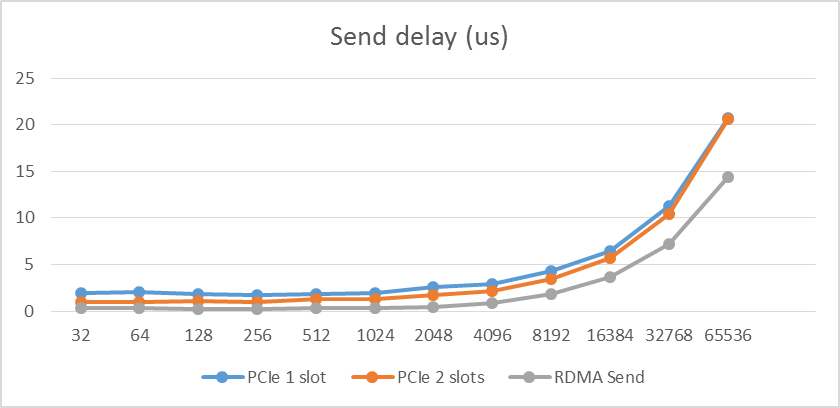
\includegraphics[width=4in]{rocelat}
\caption{RDMA Send与PCIe接口通信延迟对比} \label{fig:rocelat}
\end{figure}

\begin{figure}[htbp]
\centering
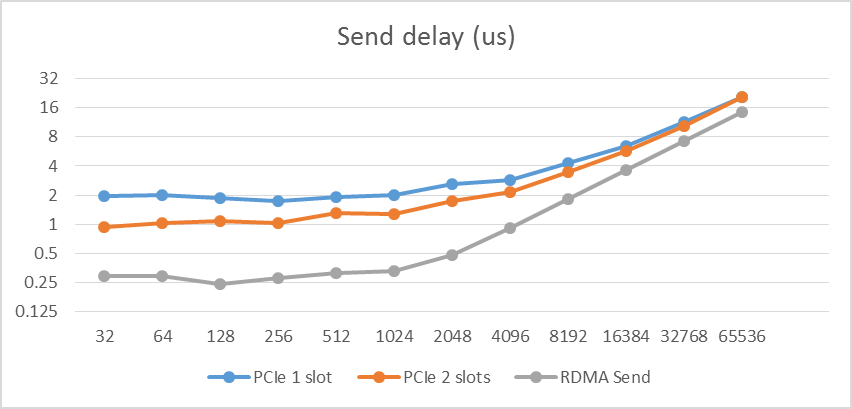
\includegraphics[width=4in]{rocelatlog}
\caption{RDMA Send与PCIe接口通信延迟对比(对数纵坐标)} \label{fig:rocelatlog}
\end{figure}

\begin{figure}[htbp]
\centering
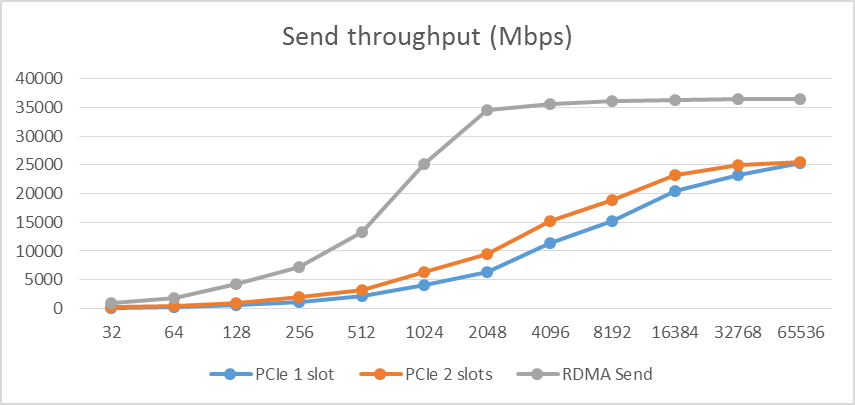
\includegraphics[width=4in]{rocerate}
\caption{RDMA Send与PCIe接口通信带宽对比} \label{fig:rocerate}
\note{实验中Send、Read、Write的性能没有明显差异,故只列出Send的数据}
\end{figure}

实验结果表明,RoCE能够有效利用网卡的通信带宽,实现比PCIe接口更高的传输速率以及更低的延迟。
使用RoCE替代PCIe通信能够提升FPGA的存储性能。
